\documentclass[twoside]{amsart}

\usepackage[brazilian]{babel}
\usepackage{csquotes}
%\usepackage[sorting=none, style=verbose-inote, backend=biber]{biblatex}
\usepackage{amsmath}
\usepackage{amssymb}
\usepackage{bbm}
\usepackage{graphics}
\usepackage{mathtools}
\usepackage[hidelinks]{hyperref}
\usepackage{physics}
\usepackage{enumitem}
\usepackage{slashed}
\usepackage[lmargin=0.5cm,rmargin=0.5cm, tmargin =1cm,bmargin =1cm]{geometry}
\usepackage[explicit]{titlesec}
\usepackage{tensor}
\usepackage{cleveref}
\usepackage{ragged2e}
\usepackage{subcaption}

\usepackage{tcolorbox}
\tcbuselibrary{minted,breakable,xparse,skins}

\definecolor{bg}{gray}{0.95}
\DeclareTCBListing{mintedbox}{O{}m!O{}}{%
  breakable=true,
  listing engine=minted,
  listing only,
  minted language=#2,
  minted style=default,
  minted options={%
    linenos,
    gobble=0,
    breaklines=true,
    breakafter=,,
    fontsize=\small,
    numbersep=8pt,
    #1},
  boxsep=0pt,
  left skip=0pt,
  right skip=0pt,
  left=25pt,
  right=0pt,
  top=3pt,
  bottom=3pt,
  arc=5pt,
  leftrule=0pt,
  rightrule=0pt,
  bottomrule=2pt,
  toprule=2pt,
  colback=bg,
  colframe=orange!70,
  enhanced,
  overlay={%
    \begin{tcbclipinterior}
    \fill[orange!20!white] (frame.south west) rectangle ([xshift=20pt]frame.north west);
    \end{tcbclipinterior}},
  #3}

\AtBeginDocument{\renewcommand*{\hbar}{{\mkern-1mu\mathchar'26\mkern-8mu\textnormal{h}}}}
\AtBeginDocument{\newcommand{\e}{\textnormal{e}}}
\AtBeginDocument{\newcommand{\im}{\textnormal{i}}}
\AtBeginDocument{\newcommand{\luz}{\textnormal{c}}}
\AtBeginDocument{\newcommand{\grav}{\textnormal{G}}}
\AtBeginDocument{\newcommand{\kb}{{\textnormal{k}_{\textnormal{B}}}}}
\newcommand{\Dd}[1]{\mathcal D #1}
\newcommand{\trp}[1]{{#1}^{\textnormal{T}}}
\newcommand{\Det}[1]{\textup{Det} #1}

\numberwithin{equation}{section}

\newtheorem{teo}{Teorema}[section]
\newtheorem{defi}{Definição}[section]
\newtheorem{lem}{Lema}[section]
\newtheorem{hip}{Hipótese}[subsection]

\pagestyle{plain}

\titleformat\section[block]
    {\bfseries\centering}
    {\Large Programa \thesection.}
    {\baselineskip}
    {\underbar{#1}}

\titleformat\subsection[block]
    {\bfseries\centering}
    {\Large \thesection.(\Alph{subsection})}
    {\baselineskip}
    {}

%\AddToHook{cmd/section/before}{\clearpage}

%\addbibresource{ref.bib}

\title
{
    \Huge EP4
}
\author
{
    \large Vicente V. Figueira, NUSP: 11809301
}
%\date{\today}

\begin{document}

\maketitle

%\tableofcontents

%%%%%%%%%%%%%%%%%%%%%%%%%%%%%%%%%%%%%%%%%%%%%%%%%%%%%%%%%%%%%

%\begin{refsection}

%\setcounter{section}{1}

\section{\Large EDOs via Euler e Runge-Kutta}

\subsection{via Euler}

A equação que desejamos resolver é,

\begin{align}
    \ddot y=\dot y+y-t^3-3t^2+7t+1\nonumber
\end{align}

Primeiramente dividimos em duas EDOs de primeira order,

\begin{align}
    \dot z&=z+y-t^3-3t^2+7t+1\equiv g\qty(t,y,z)\nonumber\\
    \dot y&=z\nonumber
\end{align}

E seguimos pelo procedimento padrão de Euler, substituir os valores iniciais e a cada passo 
calcular a correção para os próximos valores. O procedimento pode ser visto no código abaixo,

\begin{mintedbox}{python}
def fG(t, fY, fDerivadaY):
    return fDerivadaY + fY - t**3 - 3 * t**2 + 7 * t + 1

def fEuler(t, fY, fDerivadaY, vPasso):
    return fY + vPasso * fDerivadaY, fDerivadaY + vPasso * fG(t, fY, fDerivadaY)

fY0 = 0
fDerivadaY0 = -1

vPasso = 0.01

fY = fY0
fDerivadaY = fDerivadaY0

t=0

while (t<=5):

    fY, fDerivadaY = fEuler(t, fY, fDerivadaY, vPasso)
    t = t + vPasso    

print("y(5) = %f, z(5) = %f" %(fY, fDerivadaY))
print("y(5) = %f, z(5) = %f" %(5**3-5,3 * 5**2 - 1))
\end{mintedbox}

No qual já incluímos também o cálculo da solução exata `$y=t^3-t$'. O resultado do programa é,

\begin{table}[h]
    \begin{tabular}{lll}
    - &  Exata& Numérica \\\hline
    $y\qty(5)$  & 120.000000 & 85.019517 \\\hline
    $\dv{y}{t}\qty(5)$  &74.000000 & 16.726899
    \end{tabular}
\end{table}

\subsection{via RK4}

A mesma equação foi também resolvida pelo método de Runge-Kutta de 4ª ordem, seguindo a sub-rotina proposta, 
o código utilizado pode ser visto abaixo,

\begin{mintedbox}{python}
def fG(t, fY, fDerivadaY):
    return fDerivadaY + fY - t**3 - 3 * t**2 + 7*t + 1

def fRungeKutta4(t, fY, fDerivadaY, vPasso):

    k1y = vPasso*fDerivadaY
    k1z = vPasso*fG(t, fY, fDerivadaY)
    k2y = vPasso*(fDerivadaY + 0.5 * k1z)
    k2z = vPasso*fG(t + 0.5 * vPasso, fY + 0.5 * k1y, fDerivadaY + 0.5 * k1z)
    k3y = vPasso*(fDerivadaY + 0.5 * k2z)
    k3z = vPasso*(fG(t + 0.5 * vPasso, fY + 0.5 * k2y, fDerivadaY + 0.5 * k2z))
    k4y = vPasso*(fDerivadaY + k3z)
    k4z = vPasso*fG(t + vPasso, fY + k3y, fDerivadaY + k3z)

    return (k1y + 2 * (k2y + k3y) + k4y)/6, (k1z + 2 * (k2z + k3z) + k4z)/6

vPasso = 0.01

fY0 = 0
fDerivadaY0 = -1

fY = fY0
fDerivadaY = fDerivadaY0

t = 0

while (t<=5):

    vDeltaY, vDeltaDerivadaY = fRungeKutta4(t, fY, fDerivadaY, vPasso)

    fY += vDeltaY
    fDerivadaY += vDeltaDerivadaY
    
    t += vPasso

print("y(5) = %.8f, z(5) = %.8f" %(fY, fDerivadaY))
print("y(5) = %.8f, z(5) = %.8f" %(5**3 - 5, 3 * 5**2 - 1))
\end{mintedbox}

O programa devolve os valores da solução exata e da solução numérica como sendo,

\begin{table}[h]
    \begin{tabular}{lll}
    - &  Exata& Numérica \\\hline
    $y\qty(5)$  & 120.000000 & 120.74149799 \\\hline
    $\dv{y}{t}\qty(5)$  & 74.000000& 74.30029513
    \end{tabular}
\end{table}

\section{Equação de Duffing, Potencial de Poço Duplo}

\subsection{Espaço de Fase}

Utilizamo-nos do mesmo procedimento do item anterior para resolver,

\begin{align}
    \ddot x&=\frac12x\qty(1-4x^2)\nonumber
\end{align}

Utilizando RK4 para evoluir temporalmente, e plotando via pyplot, o código pode ser visto abaixo,

\begin{mintedbox}{python}
import matplotlib.pyplot as plt

def fG(t, vX):
    return 0.5 * vX * (1 - 4 * vX**2)

def fRungeKutta4(t, vX, vV, vPasso):

    k1x = vPasso * vV
    k1v = vPasso * fG(t, vX)
    k2x = vPasso * (vV + 0.5 * k1v)
    k2v = vPasso * fG(t + 0.5 * vPasso, vX + 0.5 * k1x)
    k3x = vPasso * (vV + 0.5 * k2v)
    k3v = vPasso * fG(t + 0.5 * vPasso, vX + 0.5 * k2x)
    k4x = vPasso * (vV + k3v)
    k4v = vPasso * fG(t + vPasso, vX + k3x)

    return (k1x + 2 * (k2x + k3x) + k4x)/6, (k1v + 2 * (k2v + k3v) + k4v)/6

vPasso = 0.01

vX0 = -0.5

for i in range(3):

    tX = []
    tV = []

    if i == 0:

        vV0 = 0.1

    elif i == 1:

        vV0 = 0.25

    else:

        vV0 = 0.5

    vX = vX0
    vV = vV0

    tX.append(vX)
    tV.append(vV)
    
    t = 0

    while (t<40):

        vDeltaX, vDeltaV = fRungeKutta4(t, vX, vV, vPasso)

        vX += vDeltaX
        vV += vDeltaV
        t += vPasso

        tX.append(vX)
        tV.append(vV)

    plt.plot(tX, tV, label="dot x(0) = %.2f" %vV0)

plt.title("Diagramas de espaço de fase")
plt.xlabel("$x(t)$")
plt.ylabel("$dot x(t)$")
plt.legend()
plt.show()
\end{mintedbox}

O código devolve 3 plots para os devidos casos `$\dot x\qty(0)=0.1,0.25,0.5$', que pode ser visto abaixo na Figura 
\ref{fig1},

\begin{figure}[h]
    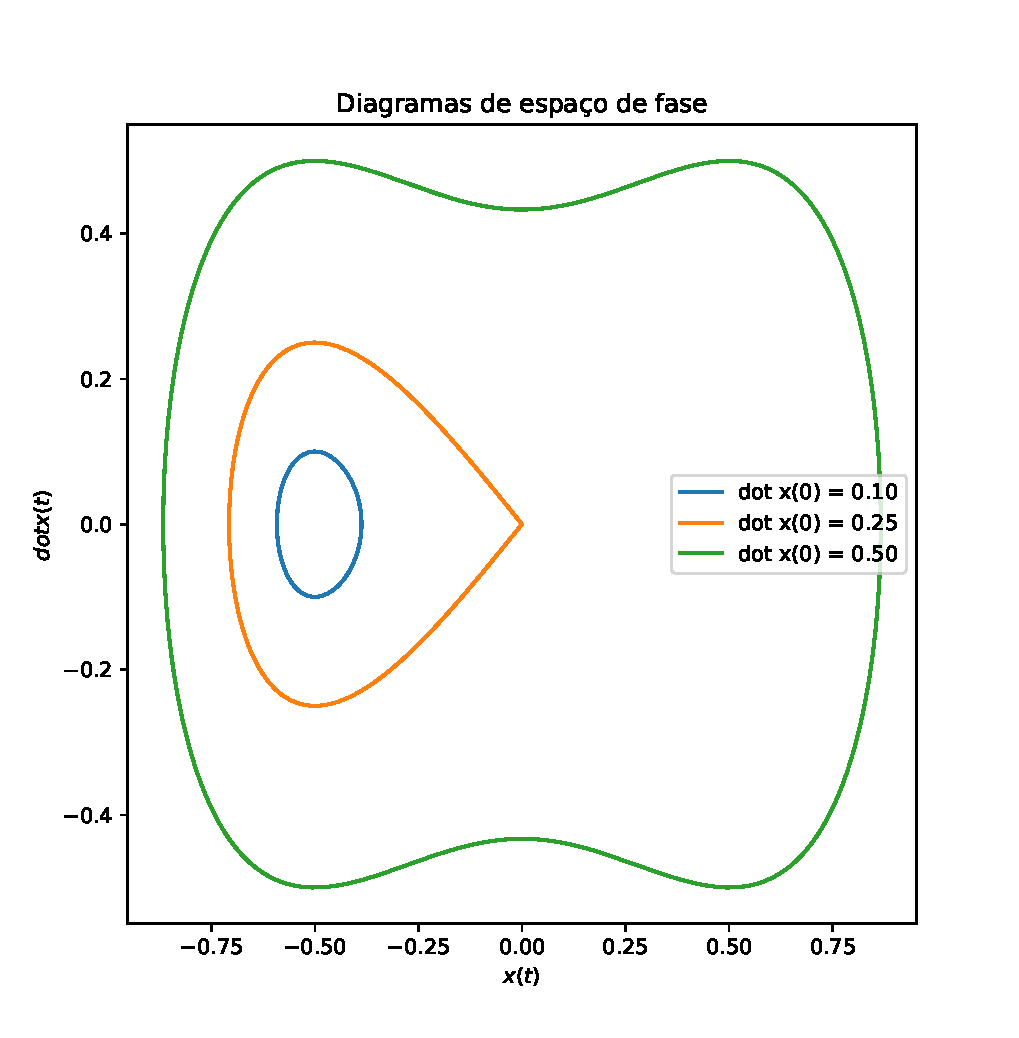
\includegraphics[width=0.5\linewidth]{II-1a.pdf}
    \caption{Evolução no espaço de fase para valores diferentes de velocidade inicial.}
    \label{fig1}
\end{figure}

Agora incluímos um amortecimento nessa equação diferencial,

\begin{align}
    \ddot{x}&=\frac12x\qty(1-4x^2)-2\dot x\gamma
\end{align}

Que é resolvido de forma similar utilizando RK4 para evoluir no espaço de fase seguindo o código,

\begin{mintedbox}{python}
import matplotlib.pyplot as plt

def fG(t, vX, vV, vGamma):
    return 0.5 * vX * (1 - 4 * vX**2) - 2 * vGamma * vV

def fRungeKutta4(t, vX, vV, vGamma, vPasso):

    k1x = vPasso * vV
    k1v = vPasso * fG(t, vX, vV, vGamma)
    k2x = vPasso * (vV + 0.5 * k1v)
    k2v = vPasso * fG(t + 0.5 * vPasso, vX + 0.5 * k1x, vV + 0.5 * k1v, vGamma)
    k3x = vPasso * (vV + 0.5 * k2v)
    k3v = vPasso * fG(t + 0.5 * vPasso, vX + 0.5 * k2x, vV + 0.5 * k2v, vGamma)
    k4x = vPasso * (vV + k3v)
    k4v = vPasso * fG(t + vPasso, vX + k3x, vV + k3v, vGamma)

    return (k1x + 2 * (k2x + k3x) + k4x)/6, (k1v + 2 * (k2v + k3v) + k4v)/6

vPasso = 0.01

vX0 = -0.5
vV0 = 0.5

tGamma = [0.25/2,0.8/2]

for vGamma in tGamma:

    tX = []
    tV = []

    vX = vX0
    vV = vV0

    tX.append(vX)
    tV.append(vV)
    
    t = 0

    while (t < 40):

        vDeltaX, vDeltaV = fRungeKutta4(t, vX, vV, vGamma, vPasso)

        vX += vDeltaX
        vV += vDeltaV

        tX.append(vX)
        tV.append(vV)

        t += vPasso

    plt.plot(tX, tV, label="2 gamma = %.2f" %(2*vGamma))

plt.title("Diagramas de espaço de fase")
plt.xlabel("$x(t)$")
plt.ylabel("$dot x(t)$")
plt.ylim(-1.1,1.1)
plt.xlim(-1.9,1.9)
plt.legend()
plt.show()
\end{mintedbox}

O código devolve um gráfico com dois plots para cada caso de `$2\gamma=0.25,0.8$', que podem sere visto abaixo na 
Figura \ref{fig2},

\begin{figure}[h]
    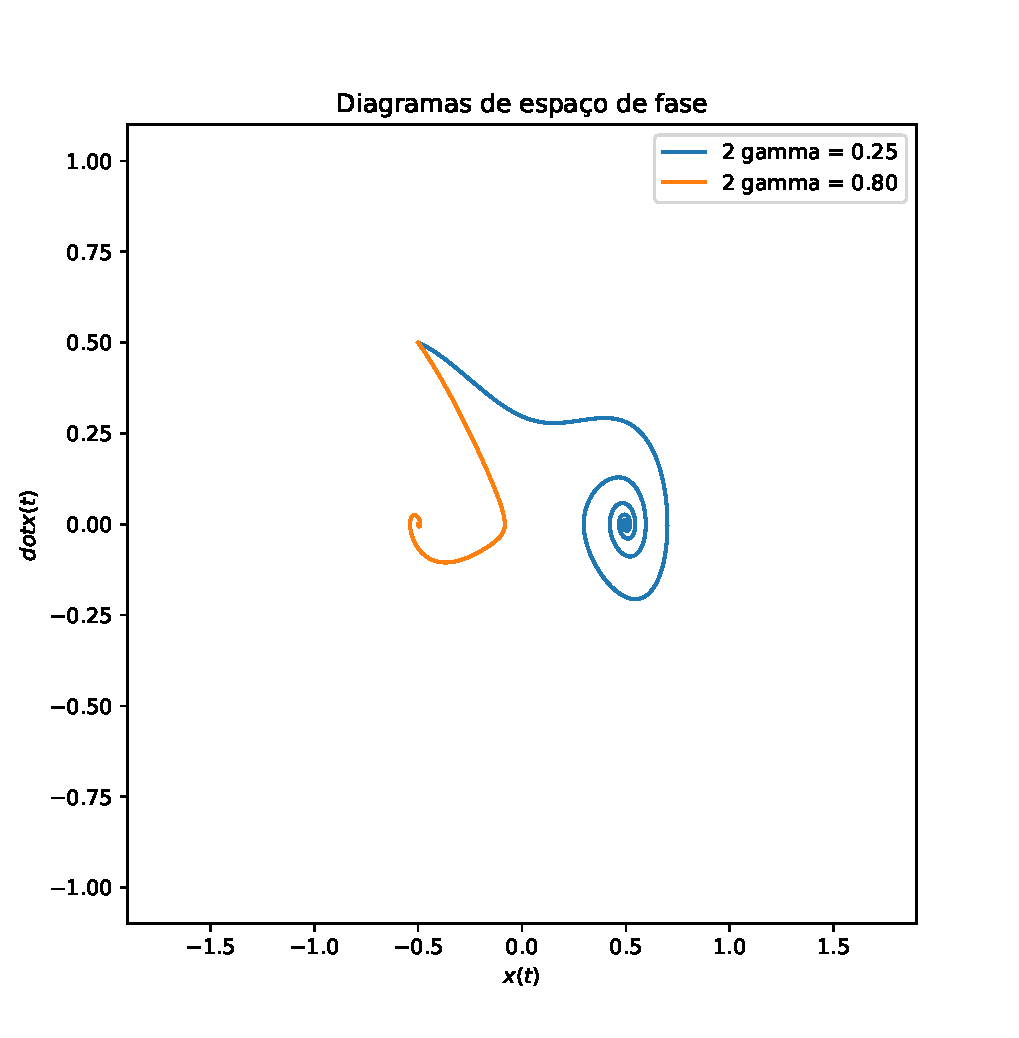
\includegraphics[width=0.5\linewidth]{II-1b.pdf}
    \caption{Evolução no espaço de fase para valores diferentes de amortecimento.}
    \label{fig2}
\end{figure}

Agora, além do amortecimento, incluímos também uma força oscilatória, 
a equação de movimento é,

\begin{align}
    \ddot x&=\frac12x\qty(1-4x^2)-\frac14\dot x+F\cos\qty(\omega t)\nonumber
\end{align}

A intensidade da Força foi variada entre os valores, `$F=0.11,0.115,0.14,0.35$'. 
Todo o processo foi novamente realizado evoluindo temporalmente o sistema no espaço 
de fase via RK4. Um detalhe a se mencionar é a remoção do transiente, 
testamos e verificamos que uma passagem de `$200000$' passos foi o suficiente para 
atingir este estágio. Partindo disto foi mais `$15000$' passos que foram 
plotados. O código que realiza esta rotina pode ser visto abaixo,

\begin{mintedbox}{python}
import numpy as np
import matplotlib.pyplot as plt

def fG(t, vX, vV, vF):
    return 0.5 * vX * (1 - 4 * vX**2) - 0.25 * vV + vF * np.cos(vOmega * t)

def fRungeKutta4(t, vX, vV, vF, vPasso, vN):

    for i in range(vN):

        k1x = vPasso * vV
        k1v = vPasso * fG(t, vX, vV, vF)
        k2x = vPasso * (vV + 0.5 * k1v)
        k2v = vPasso * fG(t + 0.5 * vPasso, vX + 0.5 * k1x, vV + 0.5 * k1v, vF)
        k3x = vPasso * (vV + 0.5 * k2v)
        k3v = vPasso * fG(t + 0.5 * vPasso, vX + 0.5 * k2x, vV + 0.5 * k2v, vF)
        k4x = vPasso * (vV + k3v)
        k4v = vPasso * fG(t + vPasso, vX + k3x, vV + k3v, vF)

        vX += (k1x + 2 * (k2x + k3x) + k4x)/6
        vV += (k1v + 2 * (k2v + k3v) + k4v)/6

        t += vPasso

    return t, vX, vV

vPasso = 0.01

vX0 = -0.5
vV0 = 0.5
vOmega = 1

tF = [0.11,0.115,0.14]

for vF in tF:

    tX = []
    tV = []

    t = 0

    t, vX, vV = fRungeKutta4(t, vX0, vV0, vF, vPasso, 200000)

    for i in range(15000):

        t, vX, vV = fRungeKutta4(t, vX, vV, vF, vPasso, 1)

        tX.append(vX)
        tV.append(vV)

    plt.plot(tX, tV, label="F = %.3f" %(vF))
    
    plt.title("Diagramas de espaço de fase")
    plt.xlabel("$x(t)$")
    plt.ylabel("$dot x(t)$")
    plt.ylim(-1.1,1.1)
    plt.xlim(-1.9,1.9)
    plt.grid()
    plt.legend()
    plt.show()
\end{mintedbox}

E os gráficos gerados podem ser vistos nas Figuras \ref{fig3}, \ref{fig4} e \ref{fig5}

\begin{figure}[h]
    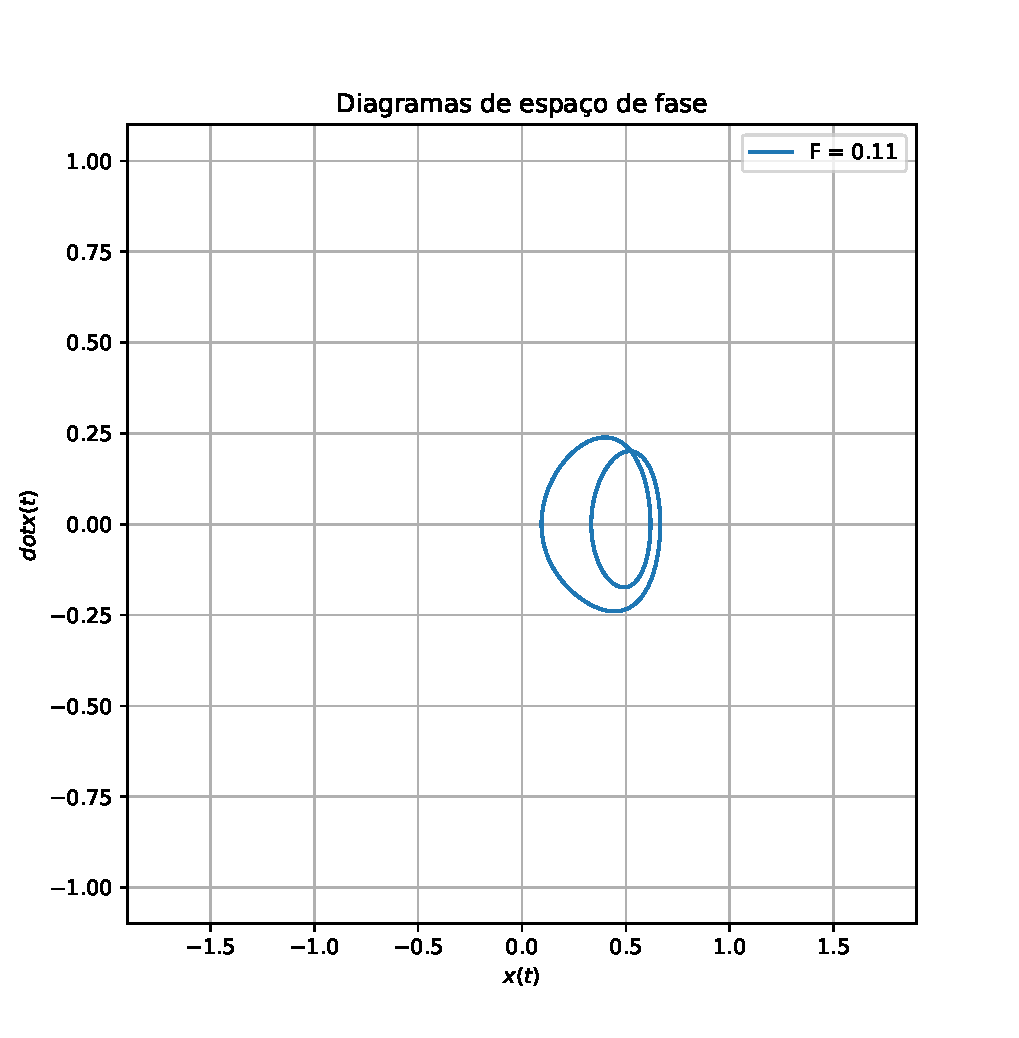
\includegraphics[width=0.5\linewidth]{II-1cf11.pdf}
    \caption{Evolução no espaço de fase para `$F=0.11$'.}
    \label{fig3}
\end{figure}

\begin{figure}[h]
    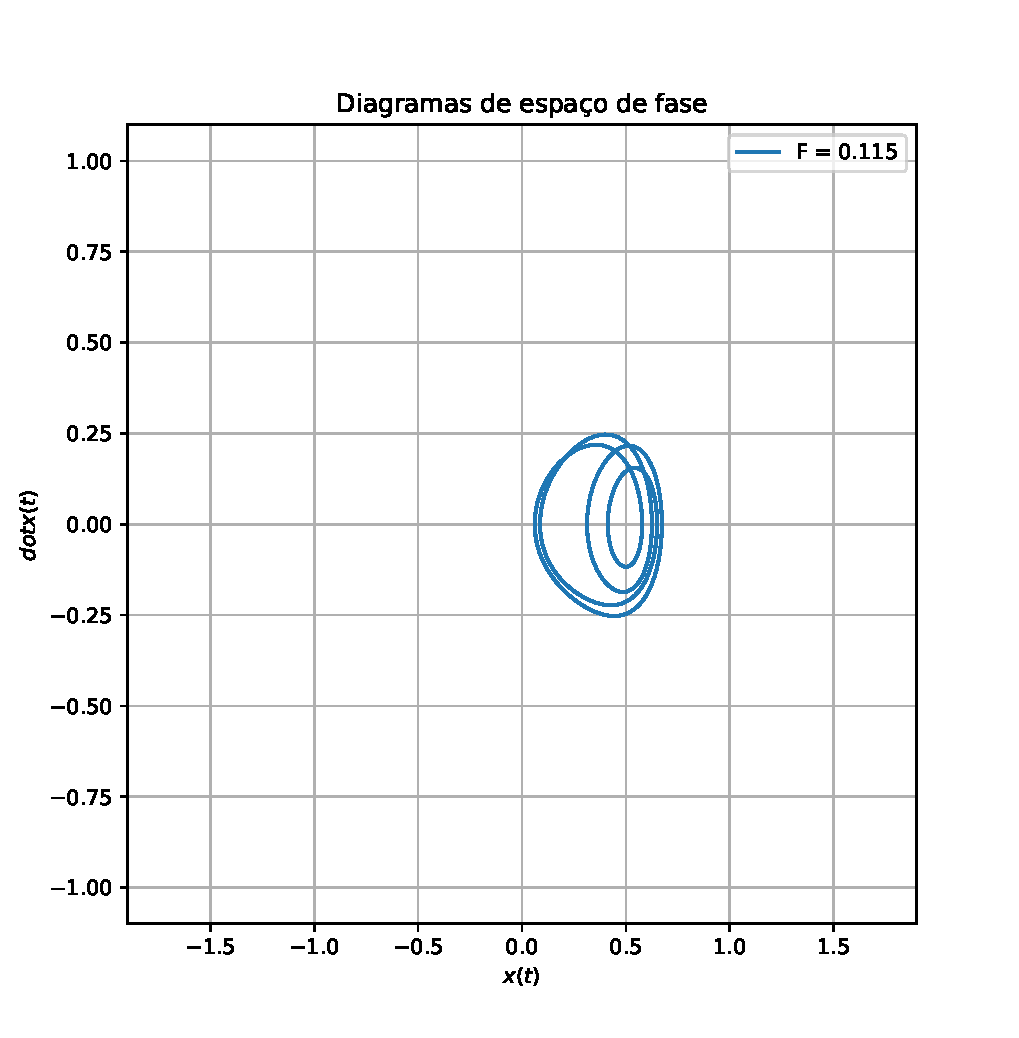
\includegraphics[width=0.5\linewidth]{II-1cf115.pdf}
    \caption{Evolução no espaço de fase para `$F=0.115$'.}
    \label{fig4}
\end{figure}

\begin{figure}[h]
    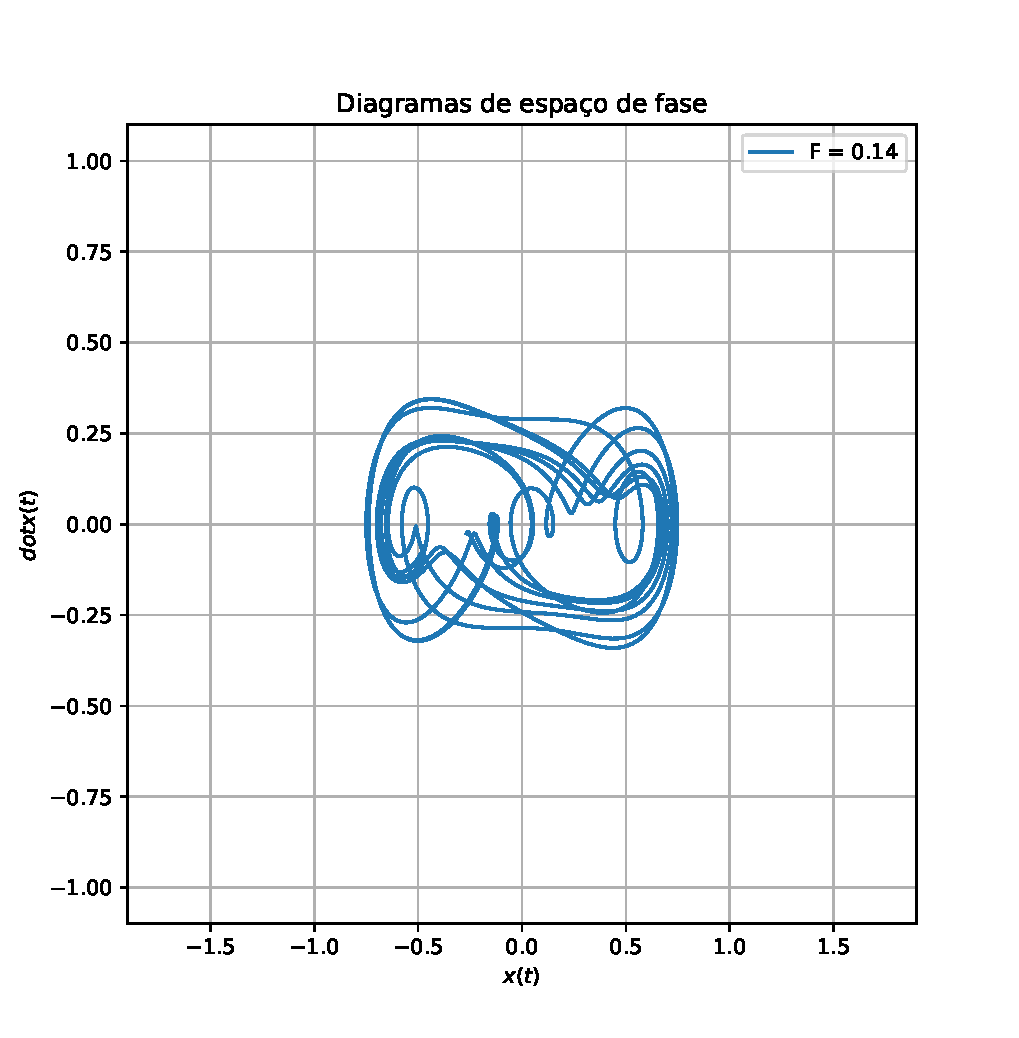
\includegraphics[width=0.5\linewidth]{II-1cf14.pdf}
    \caption{Evolução no espaço de fase para `$F=0.14$'.}
    \label{fig5}
\end{figure}

Rodamos mais uma vez o mesmo código, mas agora com `$F=0.35$', que pode ser visualizado na Figura \ref{fig6}.

\begin{figure}[h]
    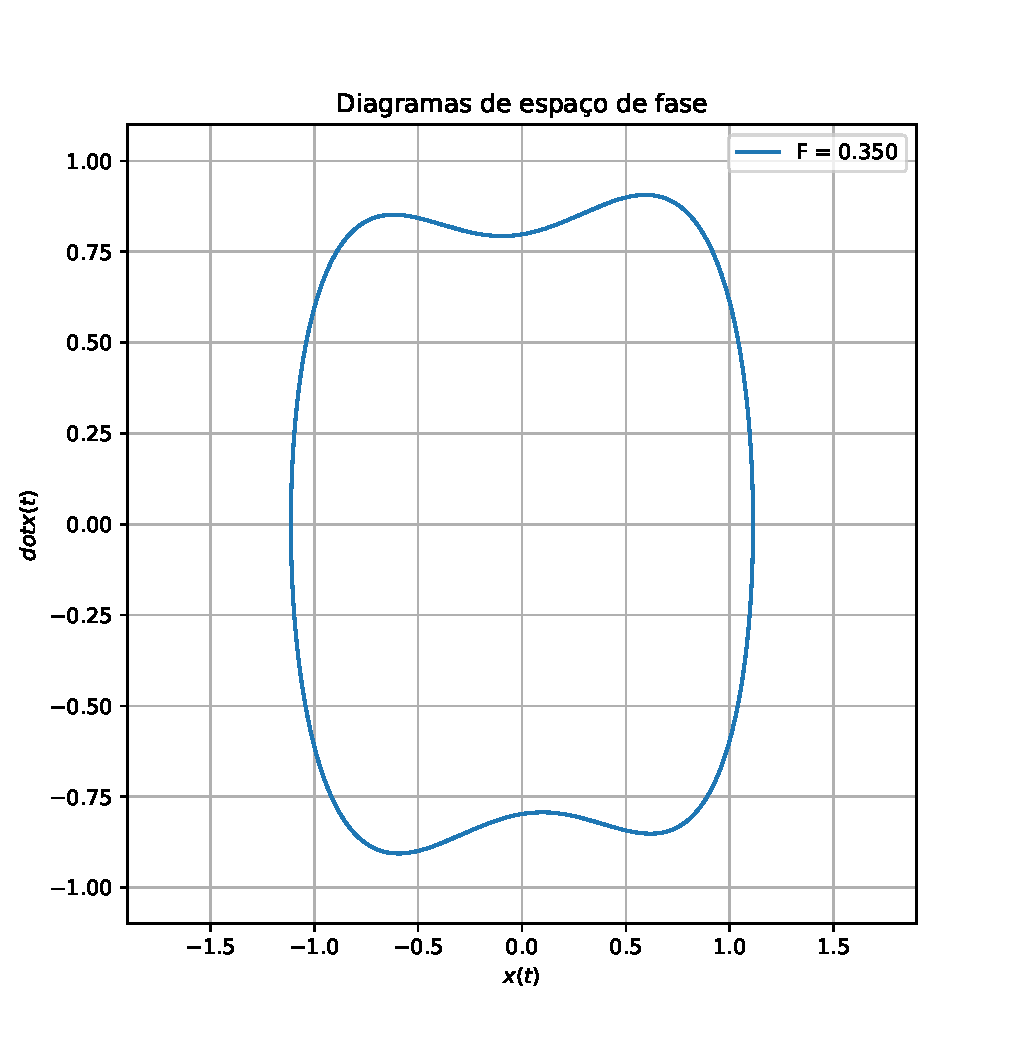
\includegraphics[width=0.5\linewidth]{II-1cf35.pdf}
    \caption{Evolução no espaço de fase para `$F=0.35$'.}
    \label{fig6}
\end{figure}

Resta-nos elaborar sobre quais são os atratores do sistema em cada uma das situações. Atratores do sistema são pontos 
em que o sistema permanece após a passagem do transiente. Assim, para a situação `$a)$', como não há amortecimento, 
toda orbita que o sistema é colocado ele permanecerá, assim, todo o espaço de fase é um atrator. Já para a situação `$b)$', 
há amortecimento, e portanto há um período de transiente, que, conforme mostrado pelos gráficos, ou acaba em `$\qty(-0.5, 0)$' 
ou em `$\qty(0.5, 0)$' dependendo da constante de amortecimento, o que implica que estes são os atratores também dependem 
destas. Para os valores calculados obtemos que para `$2\gamma=0.25$' o atrator é `$\qty(0.5,0)$' e para `$2\gamma=0.8$', o 
atrator é `$\qty(-0.5,0)$'. Já no item `$c)$', o que fizemos de eliminar o transiente por si só é calcular os atratores, 
como observamos para `$F=0.11,0.115,0.14$' o atrator é a própria figura gerada. Porém para `$F=0.14$', a trajetória no 
espaço de fase não fecha, e continua contornando proximidades dos pontos anteriores, dessa forma,o atrator ainda será um conjunto 
de pontos nas proximidades dos pontos mostrados no gráfico. Já para uma força muito grande, como o caso de `$F=0.35$', o sistema 
volta a se comportar como nas situações anteriores, a trajetória é fechada, e portanto ela mesmo é um atrator, de fato todo o espaço 
de fase é atrator neste caso, igual ao item `$a)$'.

\subsection{Diagrama de Bifurcação}

Utilizando as mesmas condições do item `$c)$', isto é,

\begin{align}
    \ddot x&=\frac12 x\qty(1-4x^2)-\dot x+ F\cos\qty(\omega t)\nonumber
\end{align}

E as condições iniciais `$x\qty(0)=-0.5;\dot x\qty(0)=0.5$', para então diferentes valores de `$F$' entre $0$ e $0.35$. Utilizamos a 
rotina proposta, usando passo de $0.00025$ para `$F$', 200000 passos para o transiente de `$0.01\frac{2\pi}{\omega}$', e 1000 passos de 
`$0.001\frac{2\pi}{\omega}$' para 100 períodos. Ao final de cada períodoo resultado obtido para `$x$' é guardado em uma lista, e no final 
fazemos um gráfico de `$x$' por `$F$'. O código utilizado pode ser visto abaixo,

\begin{mintedbox}{python}
from numpy import arange
from math import cos, pi
import matplotlib.pyplot as plt

def fG(t, vX, vV, vF):
    return 0.5 * vX * (1 -(4 * vX**2)) - 0.25 * vV + vF * cos(vFrequencia * t)

def fRK4(t, vX, vV, vF, vPasso, vN):
    for i in range(vN):

        k1x = vPasso * vV
        k1v = vPasso * fG(t, vX, vV, vF)
        k2x = vPasso * (vV + 0.5 * k1v)
        k2v = vPasso * fG(t + 0.5 * vPasso, vX + 0.5 * k1x, vV + 0.5 * k1v, vF)
        k3x = vPasso * (vV + 0.5 * k2v)
        k3v = vPasso * fG(t + 0.5 * vPasso, vX + 0.5 * k2x, vV + 0.5 * k2v, vF)
        k4x = vPasso * (vV + k3v)
        k4v = vPasso * fG(t + vPasso, vX + k3x, vV + k3v, vF)

        vX += (k1x + 2 * (k2x + k3x) + k4x)/6
        vV += (k1v + 2 * (k2v + k3v) + k4v)/6

        t += vPasso
    return t, vX, vV

vFrequencia = 1

vX0 = -0.5
vV0 = 0.5

vTransiente = 200000
vPeriodo = 1000

tX = []
tF = []

for vF in arange(0, 0.35, 25e-5):
    t = 0
    vX = vX0
    vV = vV0

    vPasso = 0.01 * 2 * pi / vFrequencia

    t, vX, vV = fRK4(t, vX, vV, vF, vPasso, vTransiente)

    vPasso = 0.001 * pi / vFrequencia

    for i in range(100):

        print("F = %f" %vF)

        t, vX, vV = fRK4(t, vX, vV, vF, vPasso, vPeriodo)

        tX.append(vX)
        tF.append(vF)

plt.scatter(tF, tX, marker='.', s = 0.3)
plt.title("Diagrama de Bifurcação")
plt.xlabel("$F$")
plt.ylabel("$x$")
plt.show()
\end{mintedbox}

O gráfico gerado pelo código pode ser visto na Figura \ref{bif},

\begin{figure}[h]
    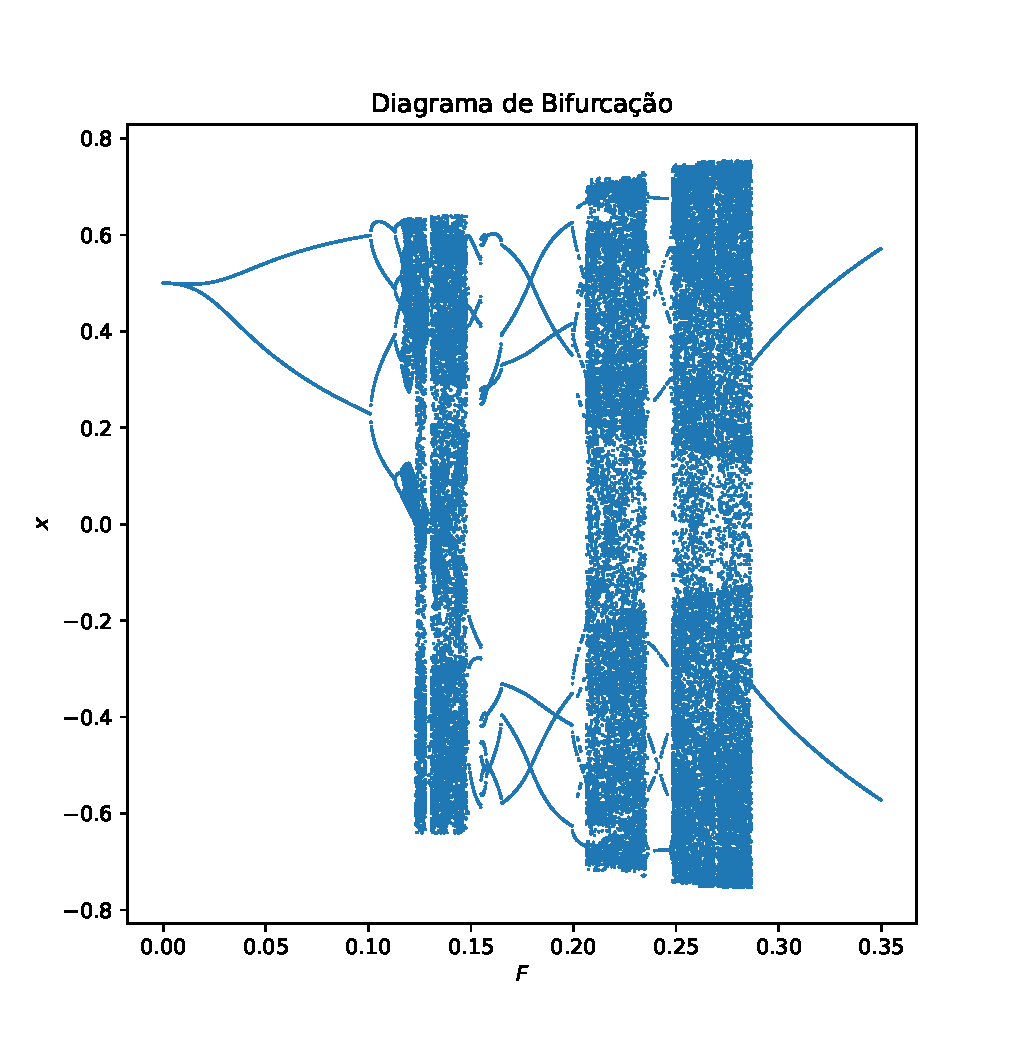
\includegraphics[width=0.5\linewidth]{bifurcaco.pdf}
    \caption{Diagrama de Bifurcação.}
    \label{bif}
\end{figure}

Onde o padrão de bifurcação é claramente visivel. Para estimar a constante de Feigenbaum, tomamos as coordenadas do 
eixo das abscissas, no nosso caso `$F$', para cada ponto de bifurcacao. Como estamos interessados apenas em uma estimativa, 
e por questões de precisão, tomamos os valores apenas das três primeiras bifurcações. Um zoom foi realizado para verificar 
a região dos dados que deveriam ser olhados, este zoom está na Figura \ref{zoom},

\begin{figure}[h]
    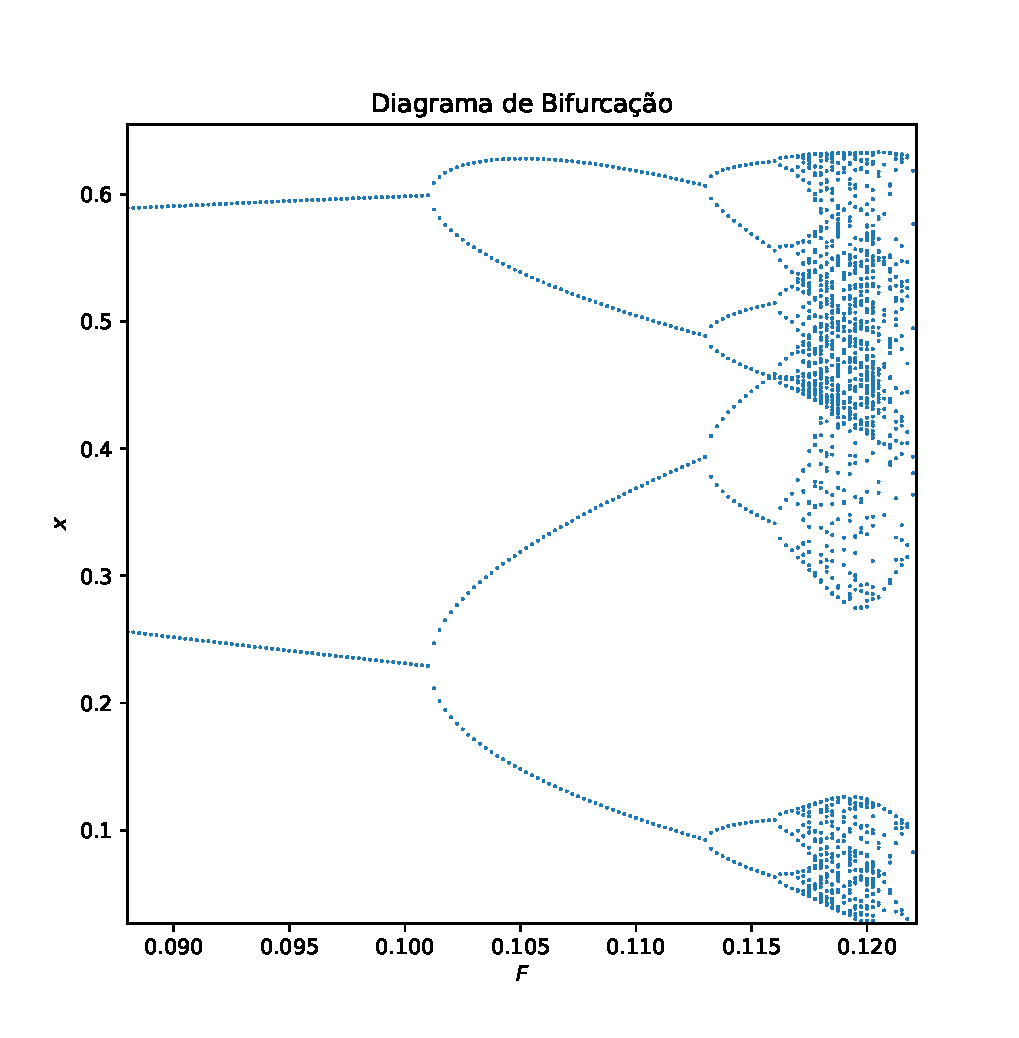
\includegraphics[width=0.5\linewidth]{bifzoom.pdf}
    \caption{Zoom do Diagrama de Bifurcação.}
    \label{zoom}
\end{figure}

A bifurcação em $0$ não foi levada em conta. Sem levar em conta esta temos,

Primeira Bifurcação: $F_1=0.10101$
Segunda Bifurcação: $F_2=0.11302$
Terceira Bifurcação: $F_3=0.11598$

Assim, a constante de Feigenbaum está relacionada com, 

\begin{align}
    \delta&=\frac{F_2-F_1}{F_3-F_2}=4.057\nonumber
\end{align}

Que é uma estimativa bem grosseria para o valor da literatura, $\delta \approx4.669201$.

\subsection{Mapa de Poincaré}

Foi utilizado o mesmo código anterior, apenas realizando as mudanças sugeridas de 
retirar o loop em `$F$', e fixar `$F=0.26$', mudando o número de períodos de $100$ para 
$20000$. O código retorna um plot de `$x$' vs `$\dot x$'. O código pode ser visto abaixo,

\begin{mintedbox}{python}
from numpy import arange
from math import cos, pi
import matplotlib.pyplot as plt

def fG(t, vX, vV, vF):
    return 0.5 * vX * (1 -(4 * vX**2)) - 0.25 * vV + vF * cos(vFrequencia * t)

def RK4(t, vX, vV, vF, vPasso, vN):
    for i in range(vN):

        k1x = vPasso * vV
        k1v = vPasso * fG(t, vX, vV, vF)
        k2x = vPasso * (vV + 0.5 * k1v)
        k2v = vPasso * fG(t + 0.5 * vPasso, vX + 0.5 * k1x, vV + 0.5 * k1v, vF)
        k3x = vPasso * (vV + 0.5 * k2v)
        k3v = vPasso * fG(t + 0.5 * vPasso, vX + 0.5 * k2x, vV + 0.5 * k2v, vF)
        k4x = vPasso * (vV + k3v)
        k4v = vPasso * fG(t + vPasso, vX + k3x, vV + k3v, vF)

        vX += (k1x + 2 * (k2x + k3x) + k4x)/6
        vV += (k1v + 2 * (k2v + k3v) + k4v)/6

        t += vPasso
    return t, vX, vV

vFrequencia = 1

vX0 = -0.5
vV0 = 0.5

vTransiente = 200000
vPeriodo = 1000

tX = []
tV = []

vF = 0.26

t = 0
vX = vX0
vV = vV0

vPasso = 0.01 * 2 * pi / vFrequencia

t, vX, vV = RK4(t, vX, vV, vF, vPasso, vTransiente)

vPasso = 0.001 * pi / vFrequencia

for i in range(20000):

    print(i)

    t, vX, vV = RK4(t, vX, vV, vF, vPasso, vPeriodo)

    tX.append(vX)
    tV.append(vV)

plt.scatter(tV, tX, marker='.', s = 0.5)
plt.title("Mapa de Poincaré")
plt.xlabel("$v$")
plt.ylabel("$x$")
plt.show()
\end{mintedbox}

E o resultado que esse renorna pode ser visto na Figura \ref{mp},

\begin{figure}[h]
    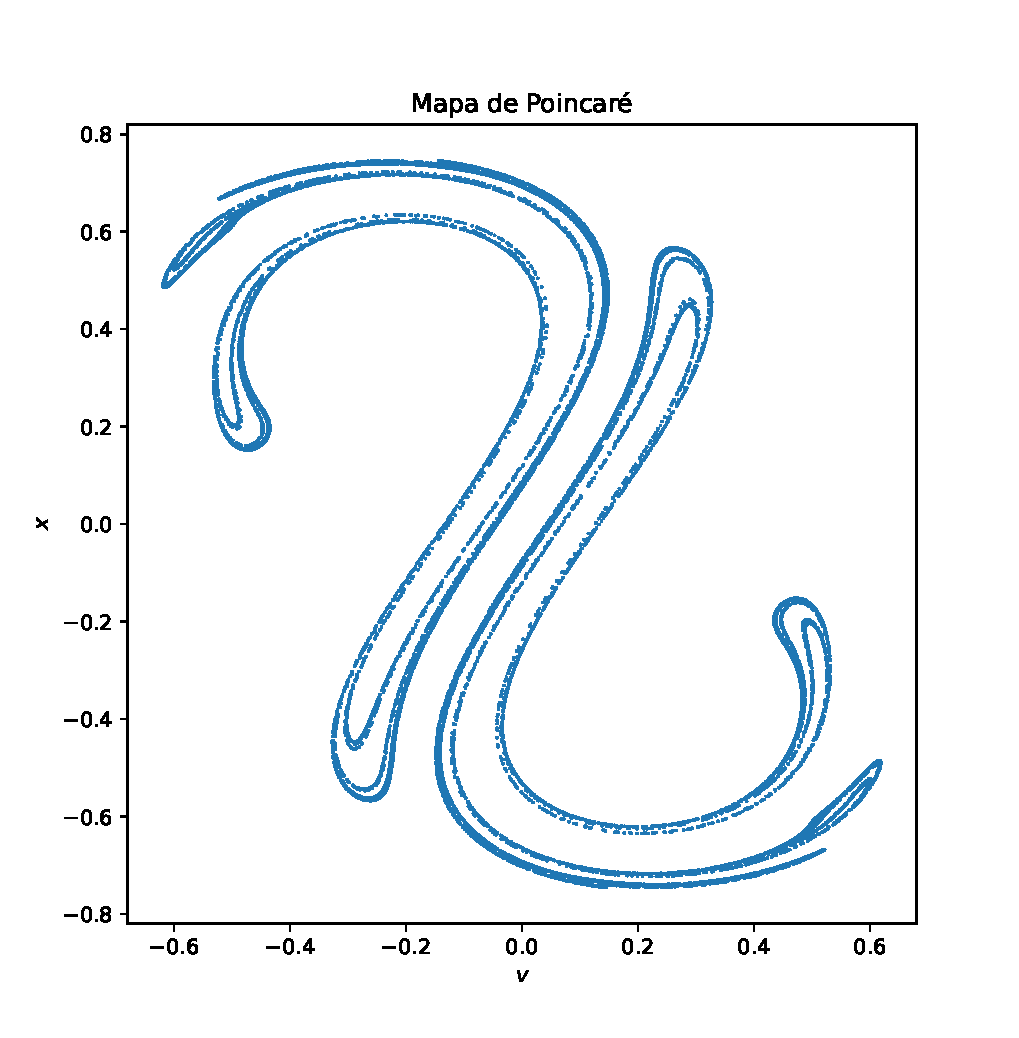
\includegraphics[width=0.5\linewidth]{mp.pdf}
    \caption{Mapa de Poincaré.}
    \label{mp}
\end{figure}

\end{document}